\chapter{L'immunité innée}\label{ch:g12:innate-immunity}

Une écharde entre dans le bout d'un doigt et en est retirée dans la
minute. Le soir, l'endroit est rouge, chaud, gonflé et lancinant~; le
lendemain, une perle de pus jaune s'est formée sous la peau~; le
troisième jour, elle a disparu. Rien n'a été décidé, rien n'a été
appris~: les mêmes quatre signes apparaissent dans toute blessure,
chez toute personne, chez tout mammifère, et le faisaient bien avant
qu'on sache qu'une écharde porte des bactéries. Ils sont la surface
visible de la première ligne de défense du corps --- un ensemble de
\omterm{def:g10:cells-common-unit:cell}{cellules} et de molécules qui reconnaissent un intrus en quelques
minutes et l'attaquent sans l'avoir jamais rencontré. Ce chapitre
décrit cette ligne~; le suivant décrit la défense plus lente, capable
d'apprendre, qu'elle appelle.

\section{Deux immunités}

\begin{definition}[Immunité innée et immunité adaptative]\label{def:g12:innate-immunity:immunity}
Le \emph{système immunitaire}\index{système immunitaire} est
l'ensemble des organes, des \omterm{def:g10:cells-common-unit:cell}{cellules} et des molécules qui défendent le
corps contre l'infection et les lésions. Il comporte deux parties.
L'\emph{immunité innée}\index{immunité innée} est présente dès la
naissance, agit en quelques minutes à quelques heures, reconnaît de
larges catégories d'intrus --- bactéries, virus, champignons, \omterm{def:g10:cells-common-unit:cell}{cellules}
abîmées --- à des traits qu'ils partagent, et répond de la même façon
à chaque fois. L'\emph{immunité adaptative}\index{immunité adaptative}
met des jours à agir, reconnaît chaque intrus individuellement, et
s'en souvient (\cref{ch:g12:adaptive-immunity}). Le système inné est
partagé par tous les animaux~; le système adaptatif n'existe que chez
les \omterm{def:g10:common-ancestry:bodyplan}{vertébrés}, et dépend du système inné pour être déclenché.
\end{definition}

\begin{proposition}[Les barrières d'abord]\label{prop:g12:innate-immunity:barriers}
La plupart des intrus n'entrent jamais. La peau, sèche, acide et
desquamant sans cesse sa surface, arrête presque tout~; les muqueuses
des voies respiratoires, de l'intestin et des voies génitales sont
humides mais tapissées d'un mucus qui piège les microbes et qui est
évacué ou renouvelé~; les larmes, la salive et le mucus portent une
\omterm{def:g11:enzymes-and-phenotype:enzyme}{enzyme} qui coupe les \omterm{def:g10:cells-common-unit:organelle}{parois bactériennes}~; l'acide de l'estomac et les
bactéries propres à l'intestin, qui occupent la place, laissent peu de
champ aux nouvelles venues. La réaction immunitaire de ce chapitre
commence quand une barrière est franchie.
\end{proposition}
\admitted

\section{La réaction inflammatoire}

\begin{proposition}[Les quatre signes et ce qui les produit]\label{prop:g12:innate-immunity:inflammation}
Une brèche --- une blessure, une infection, une brûlure --- provoque
en quelques minutes la \emph{réaction
inflammatoire}\index{inflammation}~: rougeur, chaleur, gonflement et
douleur. Chacun a sa cause~:
\begin{itemize}
  \item Des \emph{\omterm{def:g10:cells-common-unit:cell}{cellules} sentinelles} résidant dans le
        tissu --- macrophages, \omterm{prop:g12:innate-immunity:handover}{cellules dendritiques},
        mastocytes --- portent des récepteurs qui reconnaissent des
        molécules communes à des catégories entières de microbes
        (fragments de \omterm{def:g10:cells-common-unit:organelle}{parois bactériennes}, \omterm{def:g10:chemistry-of-life:families}{acides nucléiques} viraux)
        et des molécules libérées par les \omterm{def:g10:cells-common-unit:cell}{cellules} abîmées. Dès la
        reconnaissance, elles libèrent des
        \emph{médiateurs}\index{médiateur de l'inflammation}~: de
        l'histamine, des prostaglandines, et des \omterm{def:g10:chemistry-of-life:families}{protéines} de
        signalisation appelées cytokines.
  \item Les \omterm{prop:g12:innate-immunity:inflammation}{médiateurs} dilatent les vaisseaux sanguins locaux et
        rendent leur paroi perméable~: plus de sang (rougeur,
        chaleur), et du plasma qui s'infiltre dans le tissu
        (gonflement). Ils sensibilisent aussi les terminaisons
        nerveuses (douleur), et rendent la paroi des vaisseaux
        collante pour les globules blancs qui passent.
  \item Des \emph{\omterm{def:g12:innate-immunity:phagocytosis}{phagocytes}} --- des neutrophiles venus du sang en
        quelques heures, des monocytes qui deviennent macrophages en
        un jour --- se faufilent à travers la paroi des vaisseaux,
        remontent le gradient de \omterm{prop:g12:innate-immunity:inflammation}{médiateurs} jusqu'au site, et
        engloutissent et digèrent les microbes et les débris. Les
        \omterm{def:g12:innate-immunity:phagocytosis}{phagocytes} morts, les bactéries et le liquide forment le pus.
\end{itemize}
La réaction est locale, rapide, et la même pour une écharde que pour
une bactérie~: elle n'exige aucun contact antérieur avec l'intrus.
\end{proposition}
\begin{proof}[Preuves]
Injecter dans la peau un fragment de \omterm{def:g10:cells-common-unit:organelle}{paroi bactérienne} seul, sans
aucune bactérie vivante, produit en une heure la réaction complète~:
le signal est un motif moléculaire, non le microbe. Bloquer
l'histamine (avec les antihistaminiques du rhume des foins) supprime
la rougeur et le gonflement précoces~; bloquer l'\omterm{def:g11:enzymes-and-phenotype:enzyme}{enzyme} qui fabrique
les prostaglandines (avec l'aspirine ou l'ibuprofène) réduit le
gonflement, la douleur et la fièvre. Observer une blessure au
microscope montre des neutrophiles qui roulent le long de la paroi des
vaisseaux, s'arrêtent, la traversent et affluent vers le site en moins
de deux heures~; des souris privées de leurs neutrophiles meurent
d'infections qu'une souris normale règle en une nuit.
\end{proof}

\begin{omfigure}
\begin{tikzpicture}[font=\small, >=Stealth,
  b/.style={draw, rounded corners, align=center, text width=2.5cm, minimum height=1.1cm}]
  \node[b, fill=omThm!12] (breach) at (0,0) {brèche~: blessure,\\ entrée de bactéries};
  \node[b, fill=omProp!15] (sent) at (3.3,0) {cellules sentinelles~:\\ reconnaissance des\\ motifs microbiens};
  \node[b, fill=omProp!15] (med) at (6.6,0) {libération de médiateurs~:\\ histamine,\\ prostaglandines, cytokines};
  \node[b, fill=omDef!12] (ves) at (9.9,1.4) {vaisseaux dilatés\\ et perméables~: rougeur,\\ chaleur, gonflement};
  \node[b, fill=omDef!12] (nerve) at (9.9,-1.4) {terminaisons nerveuses\\ sensibilisées~: douleur};
  \node[b, fill=omMeth!15, text width=2.8cm] (phag) at (13.4,0) {les phagocytes quittent\\ le sang, engloutissent\\ les microbes~: pus};
  \draw[->, thick] (breach) -- (sent); \draw[->, thick] (sent) -- (med);
  \draw[->, thick] (med) -- (ves); \draw[->, thick] (med) -- (nerve);
  \draw[->, thick] (ves) -- (phag);
\end{tikzpicture}

{\small La \omterm{prop:g12:innate-immunity:inflammation}{réaction inflammatoire} dans l'ordre. Les \omterm{def:g10:cells-common-unit:cell}{cellules}
sentinelles détectent l'intrus à ses motifs moléculaires et libèrent
des \omterm{prop:g12:innate-immunity:inflammation}{médiateurs}~; les \omterm{prop:g12:innate-immunity:inflammation}{médiateurs} agissent sur les vaisseaux et les
nerfs, produisant les quatre signes, et appellent les \omterm{def:g12:innate-immunity:phagocytosis}{phagocytes} qui
nettoient le site.}
\end{omfigure}

\begin{omfigure}
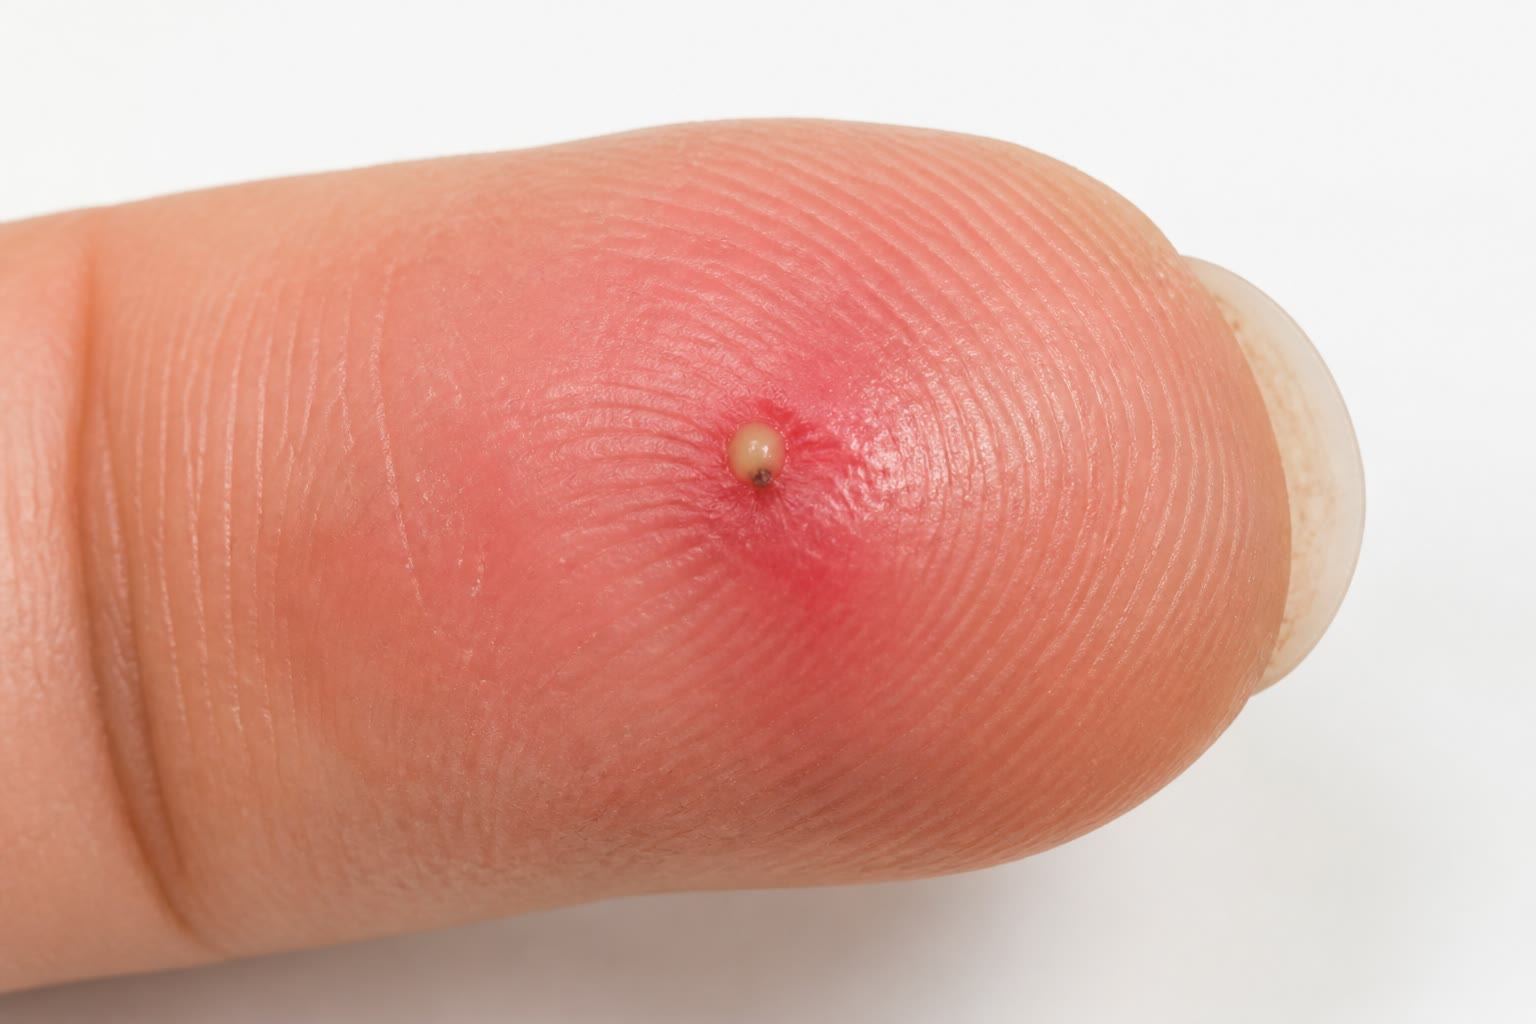
\includegraphics[width=0.56\linewidth]{images/book2/ai/g12-innate-inflamed-finger.jpg}

{\small Une blessure par écharde le lendemain~: rouge, gonflée,
douloureuse, avec une perle de pus au point d'entrée --- la \omterm{prop:g12:innate-immunity:inflammation}{réaction
inflammatoire} vue de l'extérieur. Le pus, ce sont les \omterm{def:g12:innate-immunity:phagocytosis}{phagocytes}
venus, qui ont combattu et qui sont morts.}
\end{omfigure}

\begin{definition}[Phagocytose]\label{def:g12:innate-immunity:phagocytosis}
La \emph{phagocytose}\index{phagocytose} est l'englobement d'une
particule --- une bactérie, une \omterm{def:g10:cells-common-unit:cell}{cellule} morte, un grain de
poussière --- par une \omterm{def:g10:cells-common-unit:cell}{cellule} qui enroule sa membrane autour d'elle,
la fait entrer dans une vésicule, et la digère au moyen d'\omterm{def:g11:enzymes-and-phenotype:enzyme}{enzymes} et
de composés réactifs. Les \emph{phagocytes}\index{phagocyte} de la
réaction innée sont les neutrophiles, à vie brève et nombreux, et les
macrophages, à vie longue et résidents. Un macrophage qui a digéré un
microbe garde des fragments de ses \omterm{def:g10:chemistry-of-life:families}{protéines} et les expose à sa
surface --- l'étape qui reliera cette réaction à celle du chapitre
suivant.
\end{definition}

\begin{omfigure}
\begin{tikzpicture}[font=\small, >=Stealth, line cap=round]
  \tikzset{ph/.style={draw, thick, fill=omDef!12}}
  % 1 contact
  \draw[ph] (0,0) circle (1.0); \draw[thick, fill=omThm!40, rounded corners=3pt] (1.05,-0.15) rectangle (1.75,0.15);
  \node[anchor=north, align=center] at (0.5,-1.2) {1. contact~:\\ les récepteurs lient le microbe};
  % 2 engulfing
  \begin{scope}[xshift=4.2cm]
    \draw[ph] (0,0) circle (1.0);
    \draw[thick, omDef!80!black, fill=omDef!12] (0.55,0.7) .. controls (1.5,0.6) and (1.5,-0.6) .. (0.55,-0.7);
    \draw[thick, fill=omThm!40, rounded corners=3pt] (0.75,-0.15) rectangle (1.35,0.15);
    \node[anchor=north, align=center] at (0.5,-1.2) {2. englobement~:\\ la membrane l'enveloppe};
  \end{scope}
  % 3 vesicle + digestion
  \begin{scope}[xshift=8.4cm]
    \draw[ph] (0,0) circle (1.0);
    \draw[thick, fill=white] (0.1,0.1) circle (0.42);
    \draw[thick, fill=omThm!40, rounded corners=2pt] (-0.15,0.0) rectangle (0.35,0.2);
    \foreach \a in {30,100,170,240,310} \fill[omProp] (\a:0.6) circle (1.5pt);
    \node[anchor=north, align=center] at (0,-1.2) {3. digestion dans\\ une vésicule};
  \end{scope}
  % 4 display
  \begin{scope}[xshift=12.2cm]
    \draw[ph] (0,0) circle (1.0);
    \foreach \a in {60,120,200} { \draw[thick] (\a:1.0) -- (\a:1.35); \fill[omThm] (\a:1.4) circle (2pt); }
    \node[anchor=north, align=center] at (0,-1.2) {4. fragments\\ exposés à la surface};
  \end{scope}
\end{tikzpicture}

{\small La \omterm{def:g12:innate-immunity:phagocytosis}{phagocytose}. Un \omterm{def:g12:innate-immunity:phagocytosis}{phagocyte} lie un microbe, l'enveloppe de
membrane, le digère dans une vésicule, et --- s'il s'agit d'un
macrophage ou d'une \omterm{prop:g12:innate-immunity:handover}{cellule dendritique} --- expose à sa surface des
fragments des \omterm{def:g10:chemistry-of-life:families}{protéines} du microbe à l'intention des \omterm{def:g10:cells-common-unit:cell}{cellules} de
l'\omterm{def:g12:innate-immunity:immunity}{immunité adaptative}.}
\end{omfigure}

\begin{omfigure}
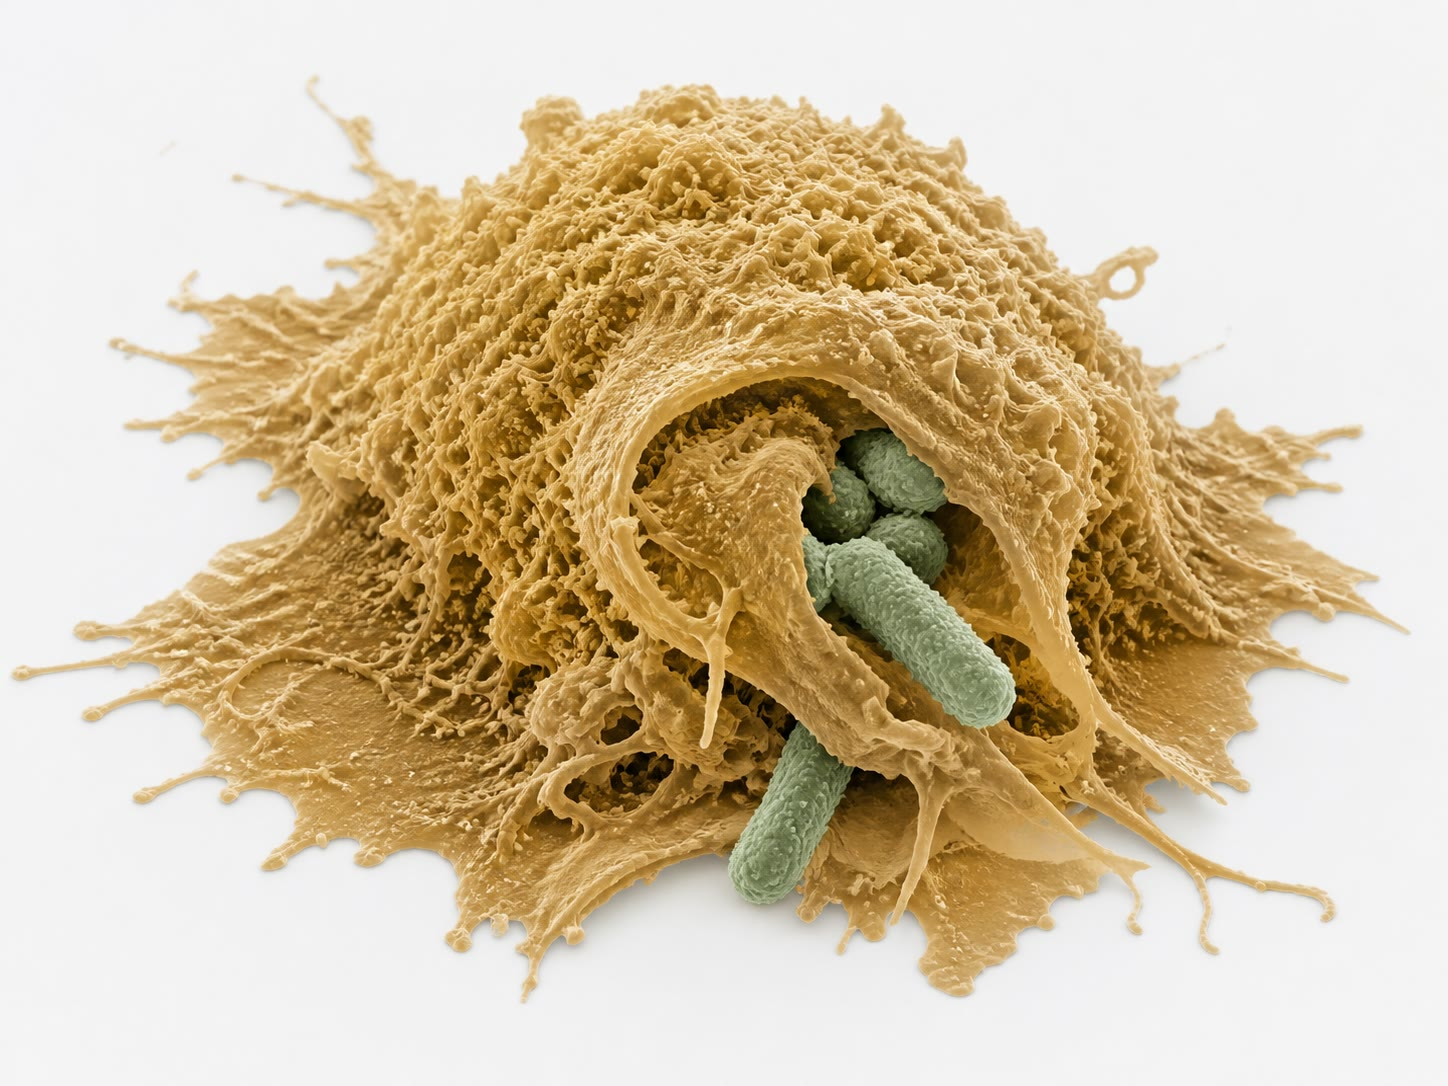
\includegraphics[width=0.56\linewidth]{images/book2/ai/g12-innate-macrophage-sem.jpg}

{\small Un macrophage, sur une micrographie électronique en fausses
couleurs, étend sa membrane autour de bactéries qu'il s'apprête à
engloutir. La \omterm{def:g10:cells-common-unit:cell}{cellule} de travail de la réaction innée.}
\end{omfigure}

\begin{example}[L'emploi du temps d'une écharde]\label{ex:g12:innate-immunity:timetable}
Minute 0~: des bactéries de l'écharde dans le tissu. Minutes 1 à 10~:
les mastocytes et les macrophages reconnaissent leurs fragments de
paroi et libèrent de l'histamine et des cytokines~; les vaisseaux se
dilatent. Heure 1~: rougeur, chaleur, les premiers neutrophiles
traversent la paroi des vaisseaux. Heures 2 à 12~: les neutrophiles
affluent, engloutissent les bactéries, meurent~; gonflement et douleur
à leur maximum. Jour 1~: les monocytes arrivent et deviennent
macrophages, nettoyant les débris~; le pus est visible. Jours 2 et 3~:
bactéries disparues, \omterm{prop:g12:innate-immunity:inflammation}{médiateurs} qui ne sont plus libérés, vaisseaux
revenus à la normale, la réparation commence. Si les bactéries se
multiplient plus vite que les \omterm{def:g12:innate-immunity:phagocytosis}{phagocytes} ne les éliminent, la réaction
s'étend, la fièvre apparaît, et la réaction adaptative --- déjà
commencée dans le ganglion lymphatique --- prend le relais.
\end{example}

\section{Calmer la réaction}

\begin{proposition}[Les anti-inflammatoires]\label{prop:g12:innate-immunity:drugs}
La \omterm{prop:g12:innate-immunity:inflammation}{réaction inflammatoire} est utile et coûteuse~: son gonflement et sa
douleur sont le prix de l'élimination de l'intrus, et lorsqu'elle est
excessive, mal dirigée (contre un pollen inoffensif, ou contre les
propres \omterm{def:g10:muscles-and-joints:joint}{articulations} du corps) ou prolongée, elle cause des dégâts
qui lui sont propres. Les
\emph{anti-inflammatoires}\index{anti-inflammatoire} agissent sur ses
\omterm{prop:g12:innate-immunity:inflammation}{médiateurs}~: l'aspirine, l'ibuprofène et leurs proches bloquent
l'\omterm{def:g11:enzymes-and-phenotype:enzyme}{enzyme} qui fabrique les prostaglandines, ce qui réduit la douleur,
le gonflement et la fièvre~; les corticoïdes, dérivés d'une \omterm{def:g11:hormones-and-reproduction:hormone}{hormone} de
la glande surrénale, éteignent la production de la plupart des
\omterm{prop:g12:innate-immunity:inflammation}{médiateurs} et servent contre les inflammations sévères ou chroniques.
Tous réduisent les signes~; aucun ne supprime la cause, et en
amortissant la réaction ils peuvent ralentir l'élimination d'une
véritable infection.
\end{proposition}
\admitted

\begin{omfigure}
\begin{tikzpicture}
\begin{axis}[
  width=0.86\linewidth, height=5.6cm,
  axis x line=bottom, axis y line=left,
  xmin=0, xmax=72, ymin=0, ymax=110,
  xlabel={heures après la blessure}, ylabel={gonflement (\% du maximum)},
  xlabel style={font=\small, at={(axis description cs:0.5,-0.12)}, anchor=north},
  ylabel style={font=\small},
  tick label style={font=\small}, xtick={0,12,24,36,48,60,72}, ytick={0,50,100},
  legend style={at={(0.97,0.95)}, anchor=north east, font=\small, draw=none},
  legend cell align=left,
]
\addplot[thick, omThm, smooth] coordinates {(0,0) (2,40) (6,85) (12,100) (24,80) (36,50) (48,25) (60,10) (72,3)};
\addplot[thick, omDef, dashed, smooth] coordinates {(0,0) (2,25) (6,45) (12,55) (24,45) (36,30) (48,15) (60,6) (72,2)};
\legend{sans traitement, avec un anti-inflammatoire}
\end{axis}
\end{tikzpicture}

{\small Le gonflement après une entorse, avec et sans
\omterm{prop:g12:innate-immunity:drugs}{anti-inflammatoire}. Le médicament réduit le gonflement de moitié en
bloquant les prostaglandines~; le déroulement de la réaction, et sa
cause, restent inchangés.}
\end{omfigure}

\begin{example}[La fièvre]\label{ex:g12:innate-immunity:fever}
Les cytokines libérées sur un foyer d'inflammation étendu ou
persistant atteignent le cerveau, où elles élèvent la valeur de
consigne de la température du corps~: c'est la fièvre. Un ou deux
degrés de chaleur en plus accélèrent les \omterm{def:g12:innate-immunity:phagocytosis}{phagocytes} et ralentissent
bien des bactéries, au prix d'énergie et d'inconfort~; au-dessus de
\qty{40}{\celsius}, le coût l'emporte sur le bénéfice, et c'est là que
servent les médicaments antipyrétiques (bloqueurs de prostaglandines).
La fièvre est une réponse régulée, non une défaillance de la
régulation.
\end{example}

\section{De l'inné à l'adaptatif}

\begin{proposition}[Le passage de relais]\label{prop:g12:innate-immunity:handover}
Parmi les \omterm{def:g10:cells-common-unit:cell}{cellules} sentinelles, les \emph{cellules
dendritiques}\index{cellule dendritique} ont une seconde tâche. Ayant
englouti l'intrus, elles quittent le tissu par les vaisseaux
lymphatiques, portant à leur surface les fragments protéiques de
celui-ci, et gagnent le \emph{ganglion lymphatique} le plus proche.
Là, elles présentent ces fragments aux lymphocytes du système
adaptatif, et les cytokines qu'elles apportent disent à ces
lymphocytes de quel genre d'intrus il s'agissait. La réaction innée ne
combat donc pas seulement les premiers jours~; elle identifie l'ennemi
et en livre le signalement. Sans ce passage de relais, aucune réaction
adaptative ne commence --- c'est pourquoi un vaccin contient, outre
l'antigène, des substances qui provoquent une petite inflammation.
\end{proposition}
\admitted

\begin{omfigure}
\begin{tikzpicture}
\begin{axis}[
  width=0.86\linewidth, height=5.6cm,
  axis x line=bottom, axis y line=left,
  xmin=0, xmax=14, ymin=0, ymax=110,
  xlabel={jours après l'infection}, ylabel={réaction (\% de son maximum)},
  xlabel style={font=\small, at={(axis description cs:0.5,-0.12)}, anchor=north},
  ylabel style={font=\small},
  tick label style={font=\small}, xtick={0,2,4,6,8,10,12,14}, ytick={0,50,100},
  legend style={at={(0.5,-0.3)}, anchor=north, legend columns=2, font=\small, draw=none},
]
\addplot[thick, omThm, smooth] coordinates {(0,0) (0.2,60) (0.5,100) (1,95) (2,80) (3,60) (4,40) (5,25) (7,10) (10,3) (14,0)};
\addplot[thick, omDef, smooth] coordinates {(0,0) (2,0) (3,3) (4,10) (5,25) (6,50) (7,75) (8,90) (9,100) (11,95) (14,80)};
\legend{réaction innée (phagocytes sur le site), réaction adaptative (anticorps dans le sang)}
\end{axis}
\end{tikzpicture}

{\small Deux réactions à une première infection. La réaction innée est
à pleine puissance en quelques heures et tient la ligne~; la réaction
adaptative, lancée par le rapport des \omterm{prop:g12:innate-immunity:handover}{cellules dendritiques}, met une
semaine à atteindre son maximum --- et, contrairement à la première,
se souviendra.}
\end{omfigure}

\begin{method}[Lire une inflammation]\label{met:g12:innate-immunity:read}
\begin{enumerate}
  \item Nommer la brèche et l'intrus probable (ou la lésion sans
        intrus~: une entorse s'enflamme aussi).
  \item Attribuer chaque signe à son \omterm{prop:g12:innate-immunity:inflammation}{médiateur} et à la modification
        des vaisseaux~: la rougeur et la chaleur à des vaisseaux
        dilatés, le gonflement à des vaisseaux perméables, la douleur
        à des nerfs sensibilisés.
  \item Repérer les \omterm{def:g10:cells-common-unit:cell}{cellules} présentes à chaque stade~: les
        sentinelles d'abord, les neutrophiles en quelques heures, les
        macrophages au bout d'un jour~; le pus comme ce qu'il en
        reste.
  \item Juger si la réaction est proportionnée~: locale et résolutive
        en quelques jours (elle fonctionne comme prévu), s'étendant
        avec de la fièvre (l'infection l'emporte, la réaction
        adaptative est nécessaire), ou dirigée contre quelque chose
        d'inoffensif ou devenue chronique (un cas pour un traitement
        \omterm{prop:g12:innate-immunity:drugs}{anti-inflammatoire}).
\end{enumerate}
\end{method}

\begin{remark}[Ancienne, rapide et sans finesse]\label{rem:g12:innate-immunity:old}
L'\omterm{def:g12:innate-immunity:immunity}{immunité innée} est l'immunité d'une éponge, d'un insecte et d'un
chêne autant que d'un humain~: les récepteurs de motifs et les
\omterm{def:g12:innate-immunity:phagocytosis}{phagocytes} sont plus anciens que les \omterm{def:g10:common-ancestry:bodyplan}{vertébrés} de plusieurs centaines
de millions d'années. Elle est rapide parce qu'elle est préparée
d'avance contre des catégories d'ennemis, et sans finesse pour la même
raison~: elle ne sait pas distinguer une bactérie d'une autre, et elle
ne peut pas s'améliorer. Le système du chapitre suivant sait faire les
deux --- mais seulement une fois que celui-ci a donné l'alarme.
\end{remark}

\section{Exercices}

\begin{exercise}[$\star$]\label{exo:g12:innate-immunity:1}
Donner trois différences entre l'\omterm{def:g12:innate-immunity:immunity}{immunité innée} et l'\omterm{def:g12:innate-immunity:immunity}{immunité
adaptative}.
\end{exercise}

\begin{exercise}[$\star$]\label{exo:g12:innate-immunity:2}
Énumérer les quatre signes de l'inflammation et la modification des
vaisseaux ou des nerfs qui est derrière chacun.
\end{exercise}

\begin{exercise}[$\star$]\label{exo:g12:innate-immunity:3}
Que reconnaissent les \omterm{def:g10:cells-common-unit:cell}{cellules} sentinelles, et que libèrent-elles~?
\end{exercise}

\begin{exercise}[$\star$]\label{exo:g12:innate-immunity:4}
Décrire la \omterm{def:g12:innate-immunity:phagocytosis}{phagocytose} en quatre étapes.
\end{exercise}

\begin{exercise}[$\star$]\label{exo:g12:innate-immunity:5}
Comment l'aspirine et l'ibuprofène réduisent-ils l'inflammation~? Que
ne font-ils pas~?
\end{exercise}

\begin{exercise}[$\star\star$]\label{exo:g12:innate-immunity:6}
D'après la figure des deux réactions, quand la réaction innée
atteint-elle son maximum, quand la réaction adaptative, et à quel jour
les deux courbes se croisent-elles~?
\end{exercise}

\begin{exercise}[$\star\star$]\label{exo:g12:innate-immunity:7}
Un fragment de \omterm{def:g10:cells-common-unit:organelle}{paroi bactérienne} injecté seul provoque la \omterm{prop:g12:innate-immunity:inflammation}{réaction
inflammatoire} complète. Que montre ce fait, et que se passerait-il
avec une injection de sérum physiologique stérile~?
\end{exercise}

\begin{exercise}[$\star\star$]\label{exo:g12:innate-immunity:8}
De quoi est fait le pus~? Pourquoi apparaît-il un jour après la
blessure plutôt qu'aussitôt~?
\end{exercise}

\begin{exercise}[$\star\star$]\label{exo:g12:innate-immunity:9}
Expliquer pourquoi un antihistaminique soulage le rhume des foins mais
ne fait rien contre les stades tardifs d'une infection bactérienne.
\end{exercise}

\begin{exercise}[$\star\star$]\label{exo:g12:innate-immunity:10}
D'après la figure du gonflement, comparer le gonflement à 12 et à 36
heures avec et sans médicament. Le médicament raccourcit-il la
réaction~?
\end{exercise}

\begin{exercise}[$\star\star$]\label{exo:g12:innate-immunity:11}
Une cheville foulée, sans blessure ni microbe, devient rouge, chaude,
gonflée et douloureuse. Expliquer ce qui a déclenché les \omterm{def:g10:cells-common-unit:cell}{cellules}
sentinelles.
\end{exercise}

\begin{exercise}[$\star\star\star$]\label{exo:g12:innate-immunity:12}
Des souris privées de neutrophiles meurent d'infections que des souris
normales règlent en une nuit~; des souris privées d'\omterm{def:g12:innate-immunity:immunity}{immunité
adaptative} y survivent mais meurent d'infections quelques semaines
plus tard. Expliquer ce que chaque résultat dit du rôle et du
calendrier des deux systèmes.
\end{exercise}

\begin{exercise}[$\star\star\star$]\label{exo:g12:innate-immunity:13}
Expliquer pourquoi un médecin peut refuser un \omterm{prop:g12:innate-immunity:drugs}{anti-inflammatoire} à un
patient atteint d'un abcès mais en prescrire un pour une arthrite, à
partir de la cause de chaque inflammation.
\end{exercise}

\begin{exercise}[$\star\star\star$]\label{exo:g12:innate-immunity:14}
Expliquer pourquoi la réaction innée ne peut pas s'améliorer au fil
des infections répétées, et pourquoi la réaction adaptative le peut,
d'après la nature de ce que chacune reconnaît.
\end{exercise}

\begin{exercise}[$\star\star\star$]\label{exo:g12:innate-immunity:15}
«~L'inflammation est une maladie.~» Discuter en un paragraphe~: quand
elle est le remède, quand elle est la maladie, et ce qui en décide.
\end{exercise}

\section{Problème~: trois jours d'une écharde}

\begin{problem}[{Problème du week-end --- une blessure suivie heure
par heure~: les cellules comptées, les médiateurs suivis, les
médicaments mis à l'épreuve, et le passage de relais au ganglion
chronométré}]
\label{pb:g12:innate-immunity:1}
Une écharde introduit environ $\num{10000}$ bactéries dans le bout
d'un doigt~; elles se divisent toutes les 40 minutes. Le tissu compte
200 macrophages résidents à moins d'un millimètre de la blessure~; les
neutrophiles commencent à arriver du sang au bout d'une heure, au
rythme de $\num{50000}$ par heure, chacun capable d'engloutir environ
20 bactéries avant de mourir.

\medskip
\noindent\textbf{Partie I --- La course.}
\begin{enumerate}
  \item Combien y aurait-il de bactéries après 2 heures, puis après 4,
        si rien ne les tuait~?
  \item Les 200 macrophages en engloutissent chacun environ 5 par
        heure. Combien en retirent-ils dans la première heure, et cela
        arrête-t-il la croissance~?
  \item À partir de l'heure 1, les neutrophiles arrivent. Combien de
        bactéries les neutrophiles de la première heure peuvent-ils
        retirer en tout~?
  \item Comparer avec la \omterm{def:g12:selection-drift-speciation:population}{population} bactérienne à l'heure 2. Qui
        l'emporte~?
  \item Vers quelle heure, en gros, la blessure est-elle nettoyée~?
        Que reste-t-il sur le site~?
\end{enumerate}

\medskip
\noindent\textbf{Partie II --- Les signes.}
\begin{enumerate}[resume]
  \item Attribuer chacun des signes --- rougeur, chaleur, gonflement,
        douleur --- à un \omterm{prop:g12:innate-immunity:inflammation}{médiateur} et à une modification des vaisseaux
        ou des nerfs.
  \item Expliquer pourquoi le gonflement aide les neutrophiles, et
        pourquoi il fait mal.
  \item Le bout du doigt lance à chaque battement de cœur. Expliquer à
        partir des vaisseaux dilatés et de la pression dans le tissu
        gonflé.
  \item Un jour plus tard, une perle de pus s'est formée. Énumérer ce
        qu'elle contient.
  \item Au troisième jour, les signes ont disparu. Qu'est-ce qui a
        arrêté la libération des \omterm{prop:g12:innate-immunity:inflammation}{médiateurs}~?
\end{enumerate}

\medskip
\noindent\textbf{Partie III --- Les médicaments.}
\begin{enumerate}[resume]
  \item Un antihistaminique est pris à l'heure 1. Quels signes
        réduit-il, et lesquels non~?
  \item De l'ibuprofène est pris à l'heure 6. Quel \omterm{prop:g12:innate-immunity:inflammation}{médiateur}
        bloque-t-il, et quels signes réduit-il~?
  \item Une crème à base de corticoïde est appliquée. Qu'advient-il du
        recrutement des neutrophiles, et quel risque en découle pour
        l'infection~?
  \item Expliquer pourquoi aucun des trois médicaments ne raccourcit
        l'infection, et lequel pourrait l'allonger.
  \item Le patient a en outre une fièvre à \qty{38.5}{\celsius}.
        Quelles molécules l'ont provoquée, et à quoi sert-elle~?
\end{enumerate}

\medskip
\noindent\textbf{Partie IV --- Le rapport.}
\begin{enumerate}[resume]
  \item Des \omterm{prop:g12:innate-immunity:handover}{cellules dendritiques} qui ont englouti des bactéries à
        l'heure 2 atteignent le ganglion lymphatique du coude à
        l'heure 20, exposant des fragments bactériens. Que
        portent-elles outre ces fragments, et à qui font-elles leur
        rapport~?
  \item D'après la figure des deux réactions, combien de jours
        passeront avant que les anticorps dirigés contre ces bactéries
        soient abondants~? Seront-ils nécessaires pour cette écharde~?
  \item Les mêmes bactéries entrent par une seconde écharde un mois
        plus tard. Laquelle des deux réactions est différente la
        seconde fois, et laquelle est identique~?
  \item Une personne née sans neutrophiles fonctionnels survit grâce à
        des \omterm{def:g11:antibiotic-resistance:antibiotic}{antibiotiques} quotidiens. Expliquer quelle partie de la
        défense les \omterm{def:g11:antibiotic-resistance:antibiotic}{antibiotiques} remplacent et laquelle ils ne
        peuvent pas remplacer.
  \item Énoncer le résultat~: l'heure à laquelle les \omterm{def:g12:innate-immunity:phagocytosis}{phagocytes}
        dépassent les bactéries, le \omterm{prop:g12:innate-immunity:inflammation}{médiateur} derrière chacun des
        quatre signes, et la \omterm{def:g10:cells-common-unit:cell}{cellule} qui porte le rapport au ganglion
        lymphatique.
\end{enumerate}
\end{problem}
